% Section owner: Dev Tyagi -- ablation studies
\section{Ablation Studies}\label{sec:ablation}
Each ablation changes one component of the LSTM hybrid and keeps everything else fixed (folds, inner validation engines, seed). Table~\ref{tab:ablation} and Fig.~\ref{fig:ablation} report the change in 5-fold CV RMSE. Before interpreting them, we measured how much a CV score moves when the \emph{same} configuration is retrained with different seeds (Table~\ref{tab:seeds}): about $\pm0.5$--$0.7$ cycles. Re-running one ablation with an identical configuration also gave 9.39 and then 9.60, because parallel floating-point arithmetic on a multi-core CPU is not bit-reproducible. We therefore treat only effects clearly larger than about 0.5 cycles as established.

\textbf{Branches.} Removing the feature branch costs $+4.46$ cycles (worse on all five folds), far beyond the noise: the engineered features are the backbone. Removing the sequence branch costs $+0.49$ (worse on four of five folds). That is consistent across folds but of the same size as seed noise, so the value of the sequence branch rests on several pieces of evidence together: this ablation, the stage-wise test results (Section~\ref{sec:test}) and the saliency analysis.

\textbf{Window length.} This ablation tests the Phase~1 hypothesis that fixed windows miss long degradation trajectories, and it is the clearest result. For the LSTM \emph{alone}, a longer history helps markedly: RMSE falls from 14.01 ($W=30$) to 11.87 ($W=50$), then rises to 12.46 at $W=80$, where 38\% of training cycles become partly padded. The hybrid barely changes (9.55, 9.49, 9.51), because its engineered features already carry the long-range context. We keep $W=30$, which gives the same accuracy at a fraction of the cost (3 versus 44 minutes of CV training at $W=80$).

\textbf{Regularisation and mask.} Dropout ($+0.12$ without it), weight decay ($-0.03$), Gaussian input noise ($+0.05$) and the padding mask ($+0.18$ without it) all change the error by less than the seed noise, so none of them can be shown to matter on its own at this data size. Early stopping is different. Its signal comes from only 7--8 inner-validation engines, and it stopped at epochs 14--30. Trained for a fixed 60 epochs, the hybrid's validation error ends within 0.05--0.4 cycles of its best value on every fold, so dropout and the learning-rate schedule are enough to prevent overfitting. For the sequence-only networks, whose validation error turned up after 7--16 epochs, early stopping remains necessary.

\textbf{Final configuration.} A single run with a fixed 60 epochs gave the lowest CV RMSE (9.20). Over three seeds, it remains better and steadier than the default ($9.73\pm0.54$ vs.\ $9.99\pm0.71$), and it was adopted for the test evaluation. The choice used only the CV folds. Averaged over seeds, the hybrid's CV RMSE is slightly behind XGBoost (9.26).

\begin{table}[t]
\centering
\small
\caption{Ablations of the LSTM hybrid (5-fold CV RMSE, one seed)}
\label{tab:ablation}
\resizebox{\columnwidth}{!}{\begin{tabular}{lcc}
\toprule
Variant & RMSE & $\Delta$ vs.\ hybrid \\
\midrule
Hybrid ($W=30$, early stopping) & 9.55 & -- \\
\midrule
Without sequence branch & 10.04 & $+0.49$ \\
Without feature branch & 14.01 & $+4.46$ \\
$W=50$ / $W=80$ & 9.49 / 9.51 & $-0.06$ / $-0.04$ \\
Without dropout & 9.67 & $+0.12$ \\
Without weight decay & 9.52 & $-0.03$ \\
Fixed 60 epochs (no early stopping) & \textbf{9.20} & $-0.36$ \\
With input noise ($\sigma=0.05$) & 9.60 & $+0.05$ \\
Without padding mask & 9.74 & $+0.18$ \\
\bottomrule
\end{tabular}}
\end{table}

\begin{table}[t]
\centering
\small
\caption{Seed variability of the hybrid's CV RMSE}
\label{tab:seeds}
\resizebox{\columnwidth}{!}{\begin{tabular}{lcccc}
\toprule
Configuration & seed 42 & seed 1 & seed 2 & mean $\pm$ std \\
\midrule
Early stopping (default) & 9.55 & 10.81 & 9.61 & $9.99\pm0.71$ \\
Fixed 60 epochs (final) & 9.20 & 10.27 & 9.71 & $\mathbf{9.73\pm0.54}$ \\
\bottomrule
\end{tabular}}
\end{table}

\begin{figure}[t]
  \centering
  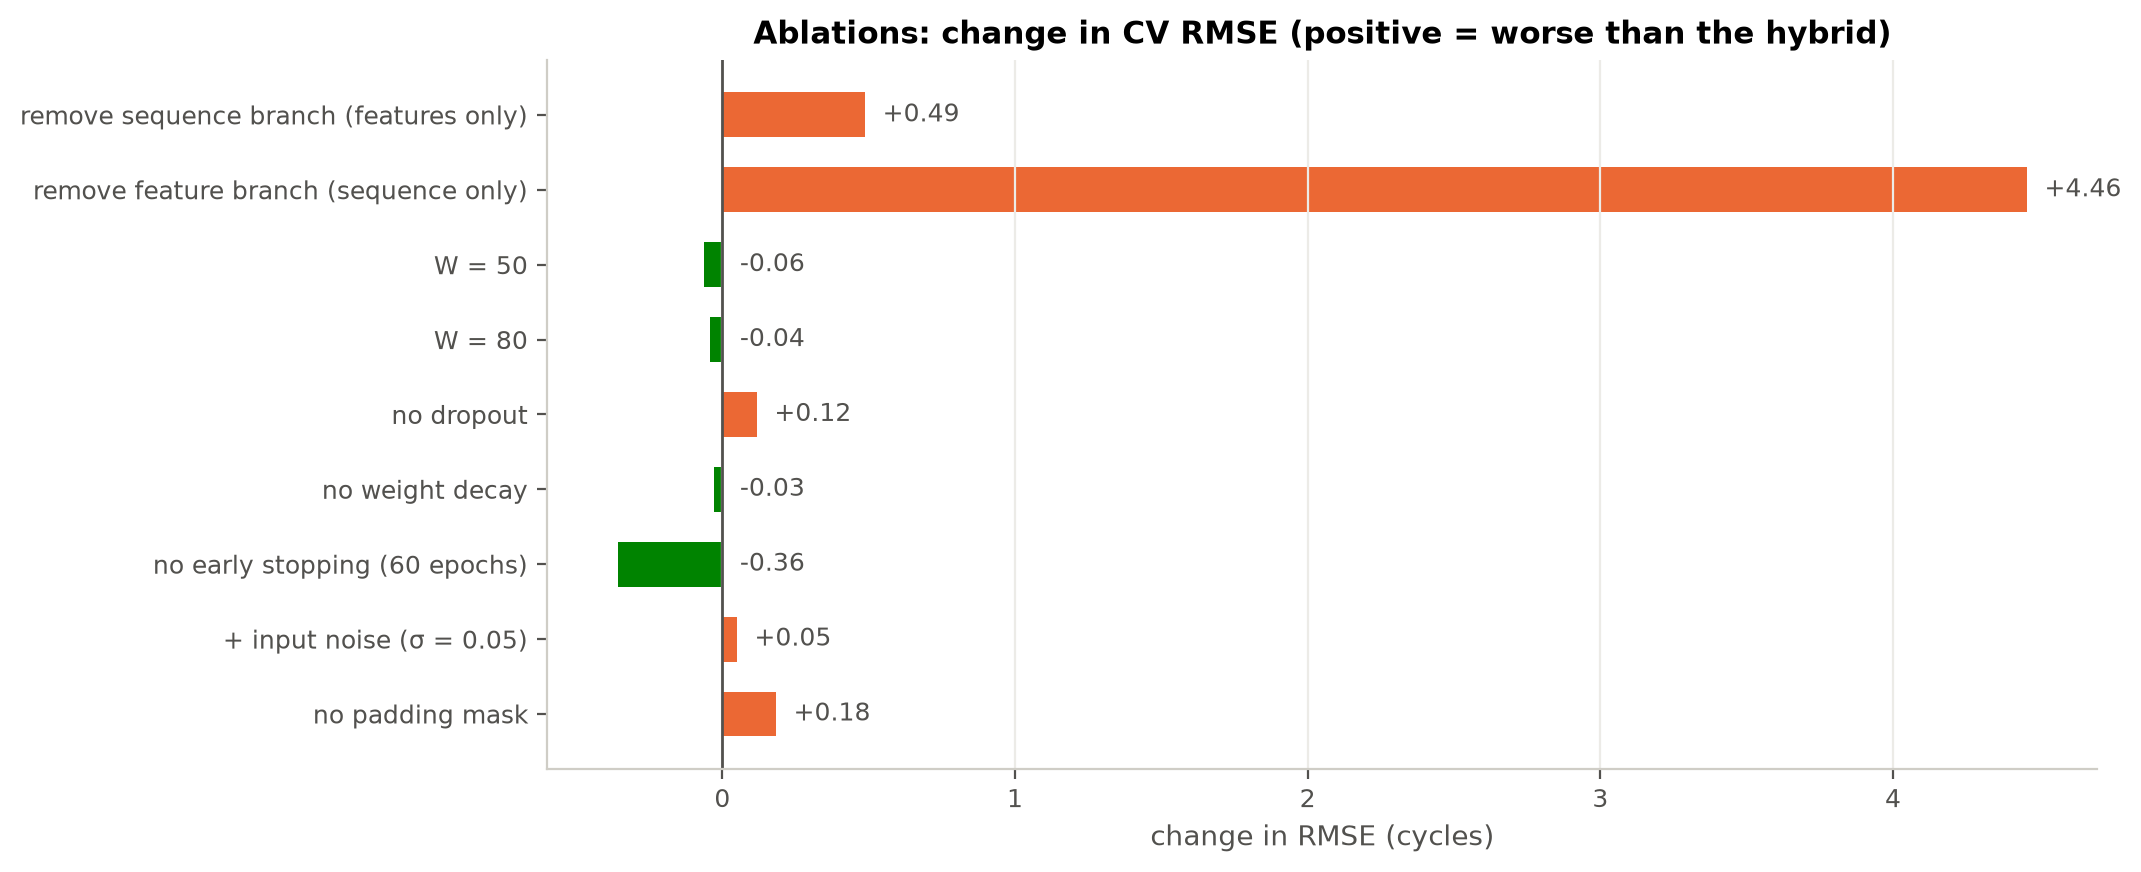
\includegraphics[width=\columnwidth]{09_ablations.png}
  \caption{Change in CV RMSE for each ablation (positive = worse). Changes below about 0.5 are within seed noise.}
  \label{fig:ablation}
\end{figure}

\begin{figure}[t]
  \centering
  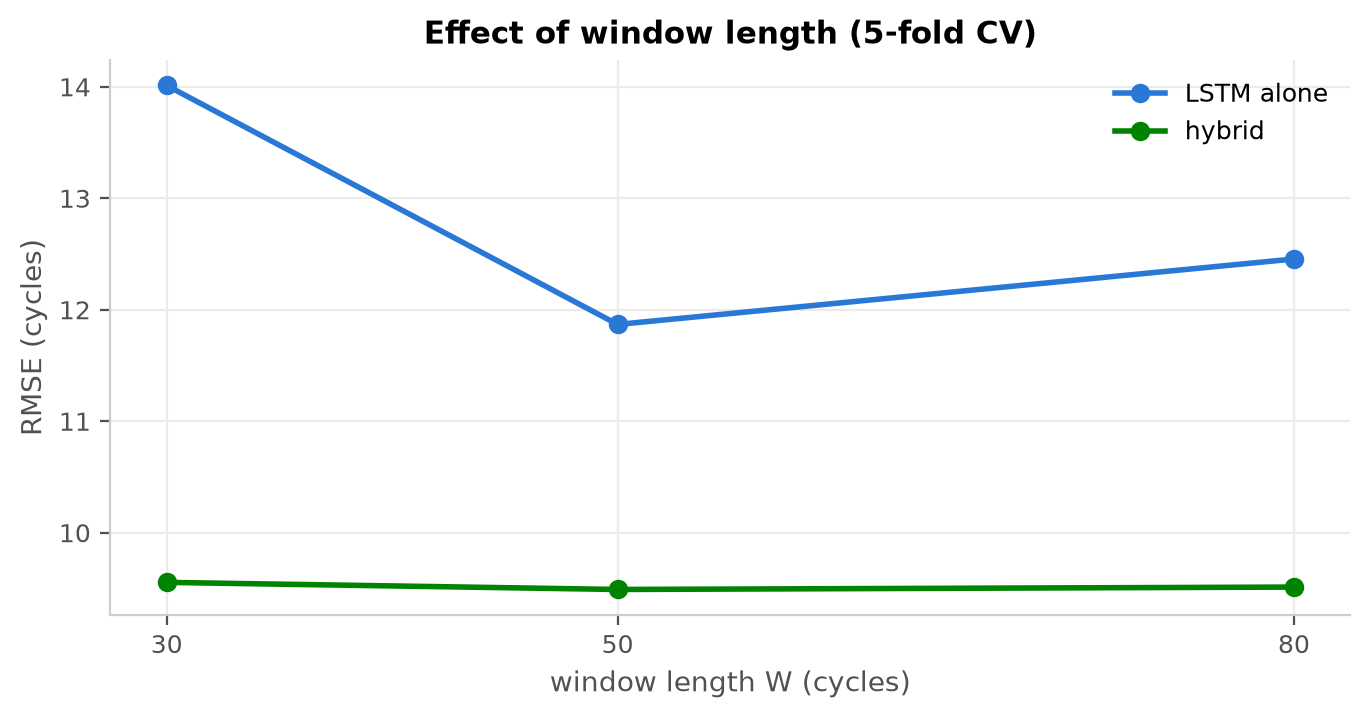
\includegraphics[width=0.8\columnwidth]{09_window_length.png}
  \caption{Window length: the sequence-only LSTM gains from longer histories; the hybrid does not need them.}
  \label{fig:window}
\end{figure}
